\input my_macros.tex
\documentclass[red]{beamer}
%\documentclass{beamer}
\mode<presentation>
{
 %	\usetheme{progressbar} 
	\usetheme{Pittsburgh}
 % \usetheme[compress]{Szeged}
	
  \usefonttheme[onlymath]{serif}
  \setbeamercovered{transparent}
}

\usepackage{kerkis} % Kerkis roman and sans

\usepackage{multimedia}
%\usepackage{movie15}
\usepackage{amsmath}
\usepackage{pgfpages}
\usepackage{xmpmulti}
\usepackage {bbm}
\usepackage[english]{babel}
\usepackage{subfigure}
\usepackage{tabularx}
\renewcommand\tabularxcolumn[1]{>{\small}m{#1}}
\newcolumntype{Y}{>{\small\centering\arraybackslash}X}
\newcolumntype{Z}{>{\small\centering\arraybackslash$}X<{$}}
\newcolumntype{W}{>{\small$}c<{$}} %For tabula




\title{Parallel Fast Gauss Transform}
\author{Shravan K. Veerapaneni}
\institute{Courant Institute of Mathematical Sciences \\
            \vspace{.1in}
%          \hspace{0.62in} \includegraphics[width = 2in]{nyu.jpg} \vspace{0.5in}   \\$\quad$}
             
\includegraphics[width = 1.3in]{nyulogo.jpg} \vspace{0.5in}   \\$\quad$}
\date{11 October 2010}             

\AtBeginSection[]
 {
   \begin{frame}<beamer>
     \frametitle{Outline}
     \tableofcontents[currentsection,hideallsubsections]
   \end{frame}
 }

\setbeamertemplate{blocks}[rounded][shadow=true]
%\setbeameroption{show notes on second screen}
\begin{document}

\begin{frame}
 \titlepage
\end{frame}

\begin{frame}
\frametitle{Outline}
\tableofcontents
\end{frame}

\section{Introduction}

\begin{frame}
\frametitle{Parallel Generalized Gauss Transforms }
\begin{block}{}
\[ 
F(x) = \int_\Omega \norm{x - y}^{2n} e^{-\frac{\norm{x - y}^2}{\delta}} f(y) \, d\Omega
 \] 
\end{block}

\begin{columns}
\begin{column}{.6\textwidth}
\begin{block}{}
\begin{itemize}
 \item Naive algorithm is $\mathcal{O}(N^2)$
 \item Extension of FGT {\tiny \texttt{(Greengard-Strain,1990)}}
 \item Works for several ``Gaussian-type'' kernels that arise from parabolic PDEs
 \item Supports highly non-uniform point distributions 
 \item 120 billion points computation in 140 sec on 4096 cores 
\end{itemize}
\end{block}
		\end{column}
		\begin{column}{.4\textwidth}
			\begin{center}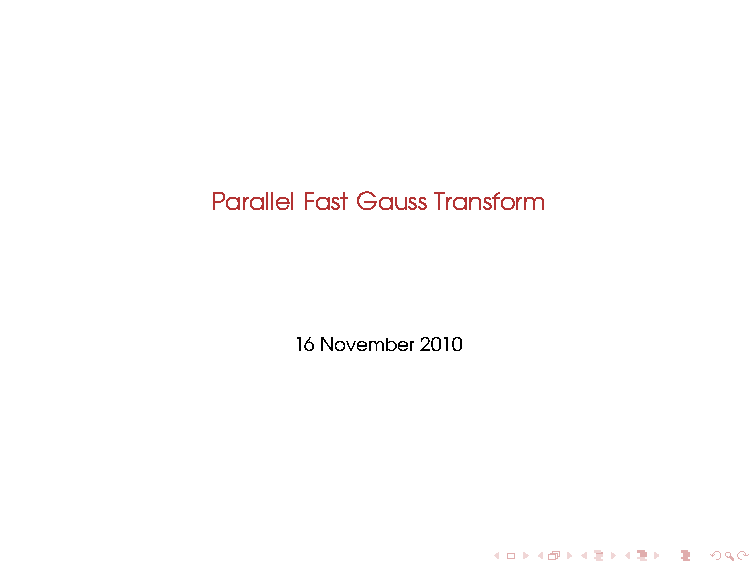
\includegraphics[width = 1.7in]{pfgt.jpg} \end{center}
		\end{column}
	\end{columns}
$\quad$\\
\texttt{{\tiny Sampath, Sundar and Veerapaneni, Supercomputing 2010 (Best Paper Award Finalist)}}		
\end{frame}



\title{Thank You !}
\author{ }
\institute{ }
\date{ }
\begin{frame}
  \titlepage
\end{frame}



\end{document}
